\documentclass[10pt,twocolumn]{article}

\usepackage[letterpaper,margin=0.72in]{geometry}
\usepackage{amsmath,amssymb,amsthm,bm}
\usepackage{booktabs}
\usepackage{graphicx}
\usepackage{xcolor}
\usepackage[hidelinks]{hyperref}
\usepackage{orcidlink}
\usepackage[numbers,sort&compress]{natbib}
\usepackage{microtype}
\usepackage{enumitem}
\usepackage{titlesec}

\graphicspath{{../../experiments/sparc_residual_dictionary/figures/}{../../experiments/sparc_nfw_residuals/figures/}}

\newcommand{\AuthorORCID}{0000-0003-1872-6179}
\newcommand{\dd}{\mathrm{d}}
\newcommand{\R}{\mathbb{R}}
\newcommand{\epsg}{\epsilon_g}
\newcommand{\Dg}{\Delta g}
\newcommand{\proj}{\Pi}

\newtheorem{theorem}{Theorem}
\newtheorem{proposition}{Proposition}
\newtheorem{remark}{Remark}

\setlength{\parindent}{0pt}
\setlength{\parskip}{2pt}
\setlength{\columnsep}{0.22in}
\setlength{\abovedisplayskip}{4pt}
\setlength{\belowdisplayskip}{4pt}
\setlength{\textfloatsep}{6pt}
\setlength{\floatsep}{5pt}
\setlength{\intextsep}{5pt}
\setlist{nosep,leftmargin=*}
\titlespacing*{\section}{0pt}{0.55ex plus 0.15ex}{0.25ex}
\titlespacing*{\subsection}{0pt}{0.45ex plus 0.1ex}{0.2ex}
\titleformat{\section}{\normalsize\bfseries}{\thesection.}{0.35em}{}
\titleformat{\subsection}{\normalsize\bfseries}{\thesubsection.}{0.35em}{}
\bibliographystyle{unsrtnat}

\title{\vspace{-1.2em}Learning Geometric Residual Structure in Galaxy Rotation Curves}
\author{
Jonathan R. Landers\\[-0.2em]
\small \orcidlink{\AuthorORCID}\,
\href{https://orcid.org/\AuthorORCID}{\AuthorORCID}\\[-0.25em]
\small Independent Researcher
}
\date{\vspace{-0.8em}}

\begin{document}
\maketitle
\vspace{-1.25em}

\begin{abstract}
Galaxy rotation curves define a noisy inverse problem: the baryonic mass model
predicts one acceleration field, while the observed dynamics imply another.
Standard analyses fit named source families, such as Navarro--Frenk--White
(NFW), cored halos, or modified-dynamics relations. This paper studies the
leftover field after such a baseline has been fit: is the remaining geometric
residual compressible across a population? We introduce a masked, smooth,
nonnegative dictionary-learning diagnostic for SPARC rotation-curve residuals.
For each galaxy we compute the baryon-subtracted acceleration residual and the
residual-of-residual left after fitting NFW to the outer region. A two-channel
lift represents signed residual fields while retaining
nonnegative coefficients. A short theorem shows that, under an idealized
baseline-projection model, residual-of-residual learning removes arbitrary
baseline variation and exactly preserves latent misspecification modes. On 131
primary-quality SPARC galaxies, a rank-six dictionary reduces held-out radial
profile error from 0.543 to 0.098 for positive acceleration residuals and from
1.075 to 0.168 for signed NFW residual-of-residuals. The same sample has a
pre-learning residual diagnostic in which cored/isothermal profiles beat NFW for
80.2\% of galaxies and outer-NFW fits leave central overshoot in 51.9\%. The
first three signed residual modes are bootstrap-stable, and a learned
coefficient is strongly associated with that independent overshoot diagnostic.
These results do not decide between dark matter and modified gravity. They show
that population residual modes are learnable model-criticism objects for the
missing-mass inverse problem.
\end{abstract}

\section{Introduction}

Flat galaxy rotation curves have long indicated that the geometry inferred from
dynamics is not the geometry predicted from observed baryons alone
\citep{Rubin1980,Bertone2018}. The usual next step is to choose a physical
source family and fit it. The dominant explanation is a non-baryonic dark
component whose halos are often modeled with the NFW profile motivated by
cold-dark-matter simulations \citep{Navarro1996,Navarro1997}.
However, disk-galaxy mass modeling also exhibits persistent small-scale
structure: cored profiles often fit individual galaxies well
\citep{Burkert1995,deBlok2010}, observed dwarf rotation curves are more diverse
than many baseline simulations predict \citep{Oman2015,Bullock2017}, and the
empirical coupling between baryonic and dynamical acceleration is striking
\citep{McGaugh2016,Famaey2012}. Recent weak-lensing analyses have further
extended the empirical reach of flat circular velocities
\citep{Mistele2024}. These facts do not imply that a simple alternative to
cold dark matter is correct. They do imply that repeated rotation-curve
residuals should be treated as structured data, not merely nuisance errors.

This paper treats the problem as a physics-constrained inverse problem
\citep{Tarantola2005}. Let
\begin{equation}
\Dg(R)=\frac{V_{\rm obs}^2(R)-V_{\rm bar}^2(R)}{R}
\end{equation}
be the weak-field acceleration residual. A named source model supplies a
candidate residual $\Dg_{\theta}(R)$; the object studied here is the leftover
field
\begin{equation}
\epsg(R)=\Dg(R)-\Dg_{\theta}(R).
\end{equation}
This is a residual-of-residual: the part of the inferred geometry not accounted
for by the chosen baseline source. The logic is conservative: fit a physical
baseline, remove it, and learn the recurring structure that remains. In that
sense $\epsg$ is a model-criticism object \citep{Gelman1996}, not a direct
theory selector.

The geometric point is that $\Dg$ is not just a scalar error bar or a
goodness-of-fit residual. In the weak-field limit it is the radial derivative
of an inferred potential perturbation, $\Dg=\dd\delta\Phi/\dd R$. Thus a
coherent pattern in $\epsg$ is a coherent leftover field after a named source
model has already been given the opportunity to explain the outer rotation
curve. The learning problem is to ask whether those leftover fields share a
low-dimensional population structure before assigning them a physical cause.

\begin{proposition}[Flat-tail residual geometry]
On a radial interval where the excess circular speed is approximately flat,
\begin{equation}
V_{\rm obs}^2(R)-V_{\rm bar}^2(R)=v_f^2 ,
\end{equation}
the residual acceleration, weak-field potential perturbation, and spherical
effective-density proxy are
\begin{align}
\Dg(R)&=\frac{v_f^2}{R},\\
\delta\Phi(R)&=v_f^2\log(R/R_0)+C,\\
\rho_{\rm eff}(R)&=\frac{v_f^2}{4\pi G R^2}.
\end{align}
\end{proposition}

\begin{proof}
The circular-speed relation gives
\begin{equation}
\Dg(R)=\frac{V_{\rm obs}^2(R)-V_{\rm bar}^2(R)}{R}
      =\frac{v_f^2}{R}.
\end{equation}
Because
\begin{equation}
\Dg(R)=\frac{\dd\delta\Phi}{\dd R},
\end{equation}
integration gives the logarithmic potential. For the spherical proxy,
\begin{equation}
M_{\rm eff}(<R)=\frac{R^2\Dg(R)}{G}
              =\frac{v_f^2R}{G},
\end{equation}
and therefore
\begin{equation}
4\pi R^2\rho_{\rm eff}(R)
=\frac{\dd M_{\rm eff}}{\dd R}
=\frac{v_f^2}{G}.
\end{equation}
\end{proof}

This elementary proposition is useful because it explains why outer rotation
curves are a hard baseline test. A profile family can match a flat tail by
approximating a logarithmic residual over a finite radial band, yet still imply
the wrong inner residual when extrapolated inward. The experiment below uses
that failure mode as a measurable diagnostic rather than as a final physical
verdict.

The machine-learning analogy is source disaggregation. In non-intrusive load
monitoring, an aggregate power trace is decomposed into latent appliance
contributions \citep{Hart1992,Kolter2012}. Here the aggregate is an irregular
radial field, and the latent components are geometric mismatch modes. Because
the profiles are sparse, uncertain, signed, and expected to be smooth, we use
dictionary learning and nonnegative matrix factorization (NMF)
\citep{LeeSeung1999,Aharon2006,Mairal2010}, not a temporal appliance model.

Contributions:
\begin{enumerate}
\item We formulate population residual learning for galaxy rotation curves as a
masked, smooth, nonnegative dictionary problem on a normalized radial grid.
\item We introduce a signed two-channel lift for residual-of-residual fields.
\item We prove a baseline-projection theorem explaining why learning
residual-of-residuals can isolate misspecification modes hidden by baseline
variation.
\item We run the method on public SPARC residuals \citep{Lelli2016}, compare
learned modes with named templates, and bootstrap mode stability.
\end{enumerate}

\section{Closest Literature}

The closest astrophysical literature is the part of halo fitting concerned with
repeated residual morphology. NFW halos provide a simulation-motivated baseline
\citep{Navarro1996,Navarro1997}, while cored profiles and observed dwarf-galaxy
diversity expose coherent departures from simple cuspy fits
\citep{Burkert1995,deBlok2010,Oman2015}. The radial acceleration relation and
MOND phenomenology emphasize the empirical coupling between baryonic and
dynamical accelerations \citep{Milgrom1983,Famaey2012,McGaugh2016}. Our
experiment does not replace these theories with a learned black box. It uses
learning to summarize the field that remains after one named baseline has been
fit.

The closest statistical literature is inverse-problem model criticism. Rotation
curves do not directly observe a source density; they observe a dynamical field
from which source models are inferred under assumptions about geometry, stellar
mass-to-light ratios, distance, inclination, and priors. Inverse-problem theory
separates the forward operator from the data-misfit object
\citep{Tarantola2005}. Posterior predictive checking similarly treats
structured discrepancies as scientific evidence about model inadequacy
\citep{Gelman1996}. The residual-of-residual $\epsg$ is a frequentist,
profile-level discrepancy designed for this purpose.

The closest machine-learning literature is additive representation learning.
NILM decomposes an aggregate power trace into appliance-level components
\citep{Hart1992,Kolter2012}. Sparse coding and dictionary learning decompose
signals into reusable atoms \citep{Olshausen1996,Aharon2006,Mairal2010}; NMF
adds nonnegativity and parts-based interpretability \citep{LeeSeung1999}. The
difference here is the observation geometry: the ``aggregate'' is an irregular
radial residual profile, and the components are population-level mismatch
modes rather than appliances.

\section{Residual Learning Setup}

\subsection{Residual profiles}

SPARC provides rotation curves and baryonic velocity components for 175 disk
galaxies \citep{Lelli2016}. We use fixed stellar mass-to-light ratios
$\Upsilon_{\rm disk}=0.5$ and $\Upsilon_{\rm bulge}=0.7$, following common
SPARC exploratory practice, and compute
\begin{equation}
V_{\rm bar}^2
=
\operatorname{sign}(V_{\rm gas})V_{\rm gas}^2
+\Upsilon_{\rm disk}V_{\rm disk}^2
+\Upsilon_{\rm bulge}V_{\rm bulge}^2 .
\end{equation}
For each usable galaxy we fit NFW, cored/isothermal, and logarithmic-tail
residual families. The dictionary experiment uses the NFW fit restricted to
the outer radial region as the baseline. This is the central stress test: if an
NFW source is forced to match the flat outer residual, does it leave coherent
inner structure behind?
This complements Bayesian SPARC halo catalogs that fit complete halo families
under priors \citep{Li2020}.

Profiles are placed on a common grid $x=R/R_d$, where $R_d$ is the SPARC disk
scale length. Each galaxy is normalized by the root-mean-square of its observed
residual so that the dictionary learns shape rather than halo scale. Let
$X\in\R^{n\times m}$ denote the nonnegative matrix for
$\max(\Dg,0)$ and let $E\in\R^{n\times m}$ denote the signed
residual-of-residual matrix. Missing entries arise because galaxies cover
different radial ranges; a mask $M$ identifies observed grid entries.

\subsection{Dictionary objectives}

For positive residuals we fit
\begin{equation}
\min_{A,\Phi\ge 0}
\sum_{ij} M_{ij}w_{ij}
\left(X_{ij}-(A\Phi)_{ij}\right)^2
+\lambda\sum_k \|\nabla_x^2\phi_k\|_2^2 ,
\label{eq:nmf}
\end{equation}
with $A\in\R_+^{n\times K}$ and $\Phi\in\R_+^{K\times m}$.
For signed residuals, we use the two-channel lift
\begin{equation}
E=E^+-E^-,
\qquad
E^\pm\ge 0,
\end{equation}
and learn a nonnegative dictionary on $[E^+,E^-]$. The decoded signed mode is
$\phi_k=\phi_k^+-\phi_k^-$. This preserves additive, nonnegative galaxy
coefficients while allowing each learned mode to have positive and negative
radial structure.

Ranks $K=1,\ldots,6$ are scored by holding out 15\% of observed radial grid
entries per split. Rank zero is the population-mean baseline. Bootstrap
stability is measured by resampling galaxies, refitting the selected
dictionary, and matching learned modes to the reference modes by absolute
profile correlation.

\subsection{Optimization protocol}

The masked objective is optimized by multiplicative NMF-style updates with
small denominators clipped for numerical stability. With Hadamard product
$\odot$ and weight matrix $W$, the positive-residual update has the form
\begin{align}
A &\leftarrow A\odot
\frac{(M\odot W\odot X)\Phi^\top}
     {(M\odot W\odot A\Phi)\Phi^\top+\varepsilon},\\
\Phi &\leftarrow \Phi\odot
\frac{A^\top(M\odot W\odot X)}
     {A^\top(M\odot W\odot A\Phi)+\varepsilon}.
\end{align}
The signed experiment applies the same updates to the lifted matrix
$[E^+,E^-]$. After each fit, mode profiles are smoothed by a second-difference
penalty, normalized, and paired with rescaled galaxy coefficients. Each rank is
fit from multiple random initializations; the seed with lowest masked training
loss is used for held-out scoring. Bootstrap refits repeat the full selection
and mode-matching procedure, so stability reflects both sample variation and
optimizer variation.

\section{Why Learn Residual-of-Residuals?}

The following idealization isolates the statistical reason for subtracting the
baseline before learning. If baseline variation is large, raw residual learning
can spend its capacity on the fitted family itself rather than on the structure
that the family missed.

\begin{theorem}[Baseline-projected residual mode identifiability]
Let $\mathcal H$ be a finite-dimensional residual-profile space, let
$\mathcal B\subset\mathcal H$ be a linear baseline subspace, and let
$\proj_{\mathcal B}$ be the orthogonal projection. For each galaxy, write
\begin{equation}
x_i=b_i+s_i+\eta_i,
\qquad
b_i\in\mathcal B,\quad s_i\in\mathcal B^\perp ,
\end{equation}
where $b_i$ is baseline variation, $s_i$ is latent misspecification, and
$\eta_i$ is noise. Define
\begin{equation}
e_i=(I-\proj_{\mathcal B})x_i .
\end{equation}

Then:
\begin{enumerate}
\item Projection removes the baseline:
\begin{equation}
e_i=s_i+(I-\proj_{\mathcal B})\eta_i .
\end{equation}
\item If $\eta_i=0$ and the misspecification has a conic dictionary
\begin{equation}
s_i=\sum_{k=1}^K a_{ik}\phi_k,
\qquad
a_{ik}\ge0,\quad \phi_k\in\mathcal B^\perp ,
\end{equation}
then the residual-of-residual has the same dictionary:
\begin{equation}
e_i=\sum_{k=1}^K a_{ik}\phi_k .
\end{equation}
\item In centered noiseless data, with row matrices $X=B+S$,
\begin{equation}
E=(I-\proj_{\mathcal B})X=S,
\qquad
\operatorname{range}(E^\top E)=\operatorname{span}\{s_i\}.
\end{equation}
The raw covariance after scaling $b_i\mapsto c b_i$ is
\begin{equation}
C_X(c)=c^2B^\top B+S^\top S .
\end{equation}
If
\begin{equation}
\alpha=\lambda_{\min}^+(B^\top B),
\qquad
\beta=\lambda_{\max}(S^\top S),
\end{equation}
then the threshold
\begin{equation}
c^2\alpha>\beta
\end{equation}
makes every nonzero baseline eigenvalue exceed every misspecification
eigenvalue. As $c\to\infty$, the leading raw eigenspace converges to the
baseline data eigenspace inside $\mathcal B$.
\end{enumerate}
\end{theorem}

\begin{proof}
Since $\proj_{\mathcal B}b_i=b_i$ and $\proj_{\mathcal B}s_i=0$,
\begin{equation}
(I-\proj_{\mathcal B})x_i
=(I-\proj_{\mathcal B})(b_i+s_i+\eta_i)
=s_i+(I-\proj_{\mathcal B})\eta_i,
\end{equation}
which proves the projection claim. The dictionary claim follows by substituting
the noiseless conic expansion for $s_i$.

For the covariance claim, center the noiseless matrices and write $X=B+S$ with
row spaces in $\mathcal B$ and $\mathcal B^\perp$. Orthogonality gives
\begin{equation}
B^\top S=S^\top B=0,
\end{equation}
so projection gives $E=S$ and
\begin{equation}
X(c)^\top X(c)=c^2B^\top B+S^\top S .
\end{equation}
This operator is block diagonal with respect to
$\mathcal B\oplus\mathcal B^\perp$, so its nonzero eigenvalues are the union of
the baseline and misspecification block eigenvalues. The condition
$c^2\alpha>\beta$ orders all nonzero baseline directions ahead of every
misspecification direction. Letting $c\to\infty$ leaves the leading raw
eigenspace in $\mathcal B$, whereas projected residual learning has already
removed $\mathcal B$.
\end{proof}

\begin{remark}
NFW fitting is nonlinear and constrained, not an orthogonal projection. The
theorem is not a claim of exact astrophysical identifiability. It is a model
criticism principle: remove the fitted baseline first, then learn the coherent
structure that remains.
\end{remark}

\section{Experiment}

\subsection{Data and preprocessing}

The experiment uses residual profiles generated by the SPARC
residual-of-residual pipeline. The mass-model table contains 3391
rotation-curve points for 175 galaxies. We use the primary-quality subset:
SPARC quality flag 1 or 2, at least eight points, and inclination above
$30^\circ$ when available. After requiring finite disk scale length and enough
normalized-radius coverage, the dictionary dataset contains 131 galaxies.

The common grid has 72 log-spaced points over
$0.25\le R/R_d\le 8.0$, with mean per-galaxy coverage 0.774. The same sample
has a central-overshoot fraction of 0.519 under the independent NFW
residual-of-residual diagnostic and a cored/isothermal-beats-NFW fraction of
0.802. These values match the earlier residual diagnostic and provide labels
for post hoc interpretation only; they are not used to train the dictionary.
Figure~\ref{fig:overshoot_diagnostic} shows the independent inner-gap
diagnostic that supplies the central-overshoot label used below.

\begin{figure*}[t]
\centering
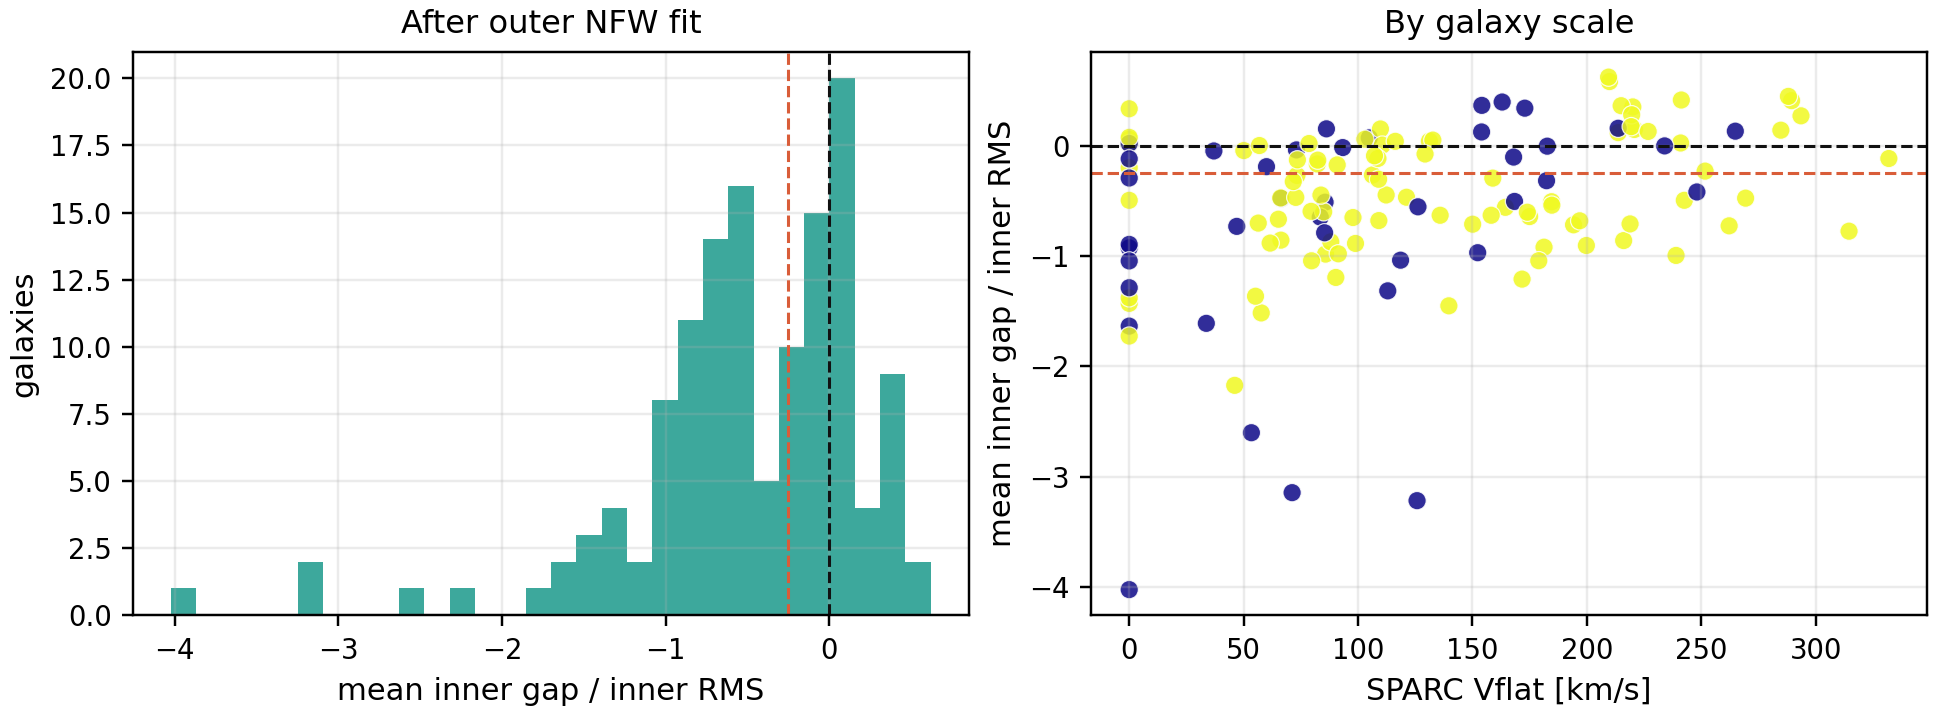
\includegraphics[width=0.90\textwidth]{central_overshoot_distribution.png}
\caption{Independent NFW residual-of-residual diagnostic for the primary-quality
SPARC sample. Left: distribution of the normalized mean inner gap after NFW has
been fit to the outer region. Right: the same diagnostic versus SPARC flat
velocity. The red dashed threshold is used only for post hoc interpretation of
learned dictionary coefficients.}
\label{fig:overshoot_diagnostic}
\end{figure*}

\begin{table}[t]
\centering
\caption{Dataset summary for the dictionary experiment.}
\label{tab:data}
\begin{tabular}{lc}
\toprule
Quantity & Value \\
\midrule
SPARC rotation-curve points & 3391 \\
Public SPARC galaxies & 175 \\
Dictionary-quality galaxies & 131 \\
Normalized radial grid points & 72 \\
Mean observed grid coverage & 0.774 \\
Central-overshoot fraction & 0.519 \\
Cored/isothermal beats NFW & 0.802 \\
\bottomrule
\end{tabular}
\end{table}

\subsection{Evaluation}

For each rank, five random radial holdout splits are used. The score reported
below is normalized profile RMSE on held-out entries after decoding signed
two-channel predictions. We also report bootstrap mode stability: 40 bootstrap
resamples of galaxies are refit, and modes are matched by absolute correlation.
Template correlations compare learned modes with simple NFW-like, cored,
central, outer-tail, and overshoot templates.

\section{Results}

\begin{table}[t]
\centering
\caption{Held-out radial-point reconstruction. Rank zero is the population
mean; $K=6$ is the largest searched rank and was selected by held-out error.}
\label{tab:heldout}
\begin{tabular}{lccc}
\toprule
Target & Baseline & $K=6$ & Improvement \\
\midrule
$\max(\Dg,0)$ & 0.543 & 0.098 & $5.5\times$ \\
$\epsg$ signed & 1.075 & 0.168 & $6.4\times$ \\
\bottomrule
\end{tabular}
\end{table}

Table~\ref{tab:heldout} gives the main compression result. The learned
dictionary substantially outperforms the population-mean baseline for both
positive residual profiles and signed NFW residual-of-residual profiles. The
model-selection curve in Fig.~\ref{fig:model_selection} decreases monotonically
through $K=6$, so the experiment demonstrates compressible population structure
rather than a sharp intrinsic rank. The selected rank should therefore be read
as a useful search endpoint, not as a claim that galaxy residuals have exactly
six physical components.

\begin{figure}[t]
\centering
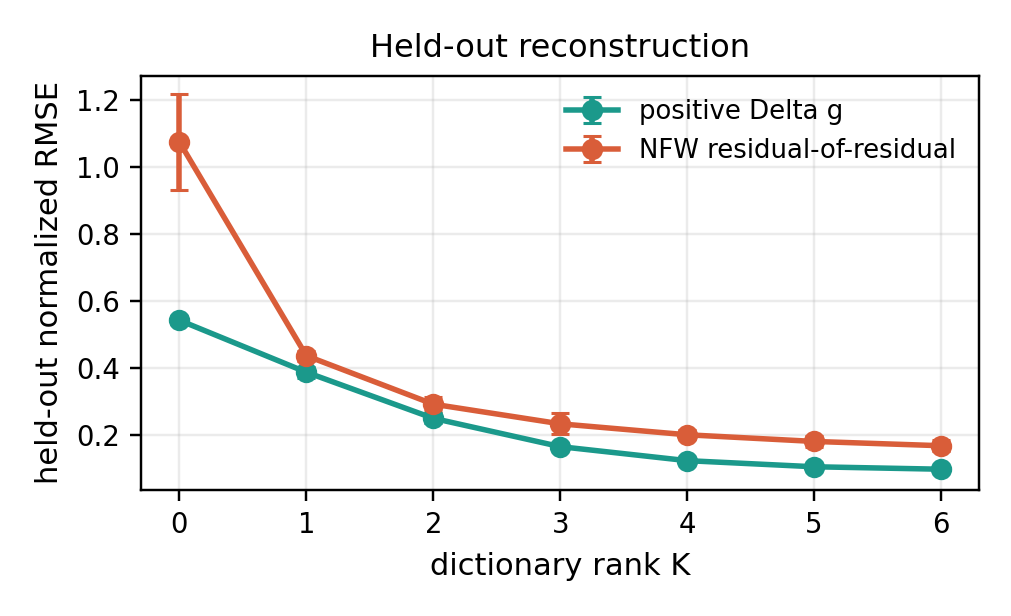
\includegraphics[width=\linewidth]{model_selection.png}
\caption{Held-out radial-point reconstruction as a function of dictionary
rank. Both targets improve through the largest searched rank, indicating
compressible residual structure without a clear elbow.}
\label{fig:model_selection}
\end{figure}

\begin{figure*}[t]
\centering
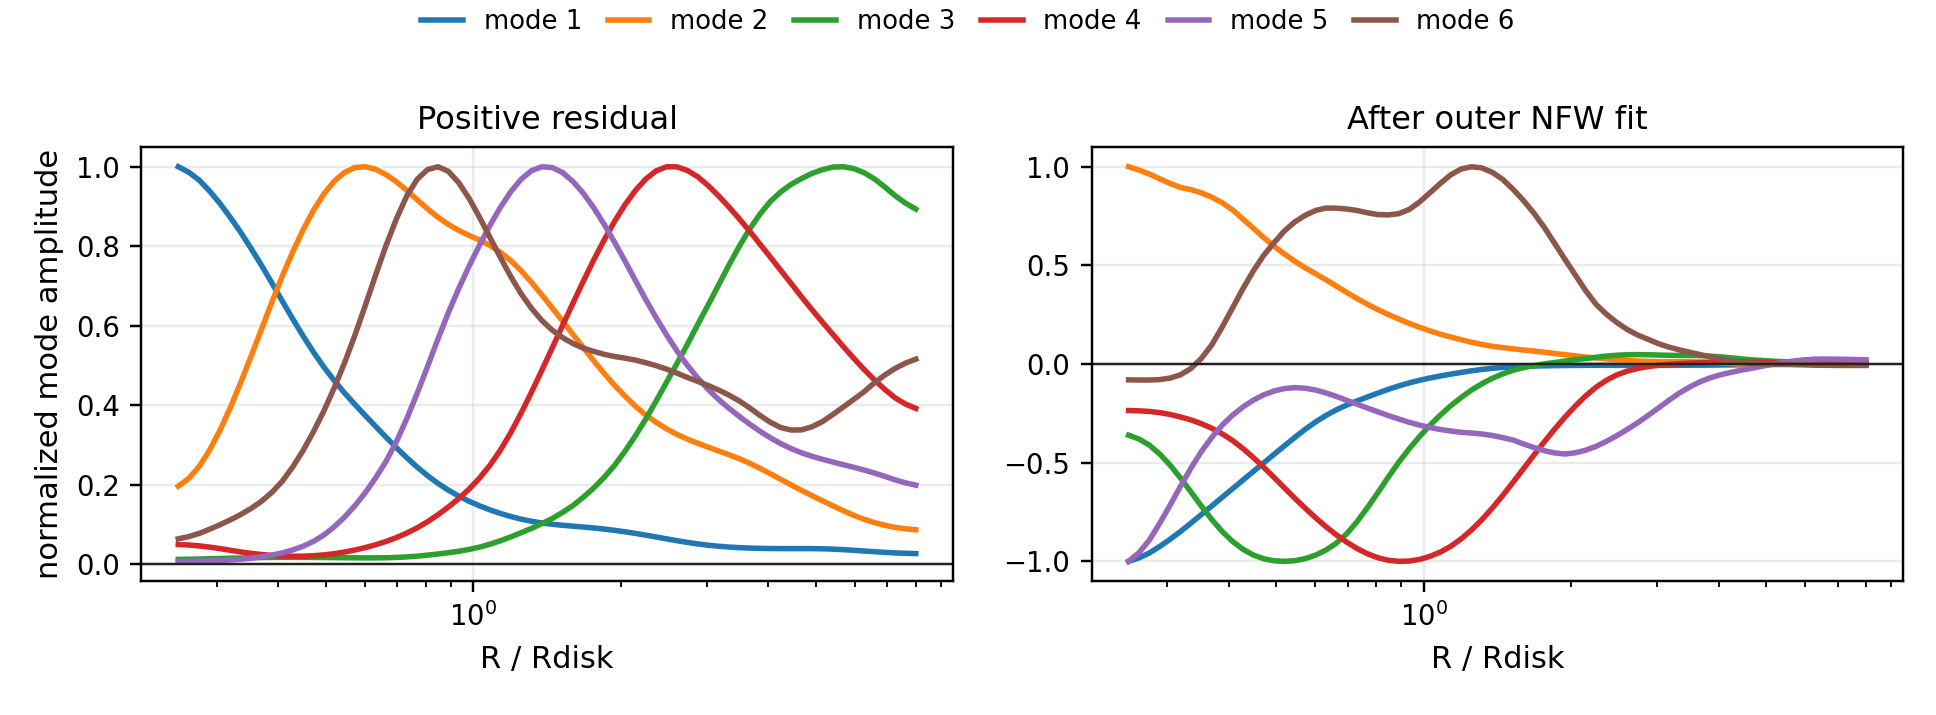
\includegraphics[width=0.92\textwidth]{learned_modes.png}
\caption{Learned population modes. Left: positive observed acceleration
residual modes. Right: signed residual-of-residual modes after fitting NFW to
the outer region. The signed modes are the more diagnostic object because they
describe what remains after a physical baseline has been forced to match the
outer residual.}
\label{fig:modes}
\end{figure*}

The learned modes in Fig.~\ref{fig:modes} make the compression result
interpretable. The positive-residual dictionary contains central, broad-tail,
and cored-like components. The signed residual-of-residual dictionary contains
several negative-inner-overshoot modes: cases where the NFW source required by
the outer residual overpredicts the inner residual. Template matching confirms
this: signed modes 1 and 3 correlate with a
negative-inner-overshoot template at 0.869 and 0.877, while mode 2 matches the
opposite sign of the same template with absolute correlation 0.936.

\begin{table}[t]
\centering
\caption{Mode-level interpretation for the signed residual-of-residual
dictionary. Correlations are post hoc diagnostics, not training labels.}
\label{tab:modeinterp}
\begin{tabular}{clc}
\toprule
Mode & Main empirical association & Value \\
\midrule
1 & Negative inner overshoot template & 0.869 \\
2 & Sign-reversed overshoot template & 0.936 \\
3 & Negative inner overshoot template & 0.877 \\
4 & Central-overshoot flag & 0.413 \\
4 & Normalized inner gap & $-0.592$ \\
6 & Central-overshoot flag & $-0.371$ \\
\bottomrule
\end{tabular}
\end{table}

\begin{table}[t]
\centering
\caption{Bootstrap stability of selected signed residual-of-residual modes.
Values are median absolute correlations to matched reference modes, with 10th
and 90th percentiles in parentheses.}
\label{tab:bootstrap}
\begin{tabular}{lccc}
\toprule
Mode & Median & 10th pct. & 90th pct. \\
\midrule
1 & 0.997 & 0.967 & 1.000 \\
2 & 0.967 & 0.838 & 0.996 \\
3 & 0.976 & 0.919 & 0.997 \\
4 & 0.846 & 0.593 & 0.987 \\
5 & 0.684 & 0.579 & 0.858 \\
6 & 0.890 & 0.626 & 0.949 \\
\bottomrule
\end{tabular}
\end{table}

The first three signed modes are highly stable under galaxy bootstrap
(Table~\ref{tab:bootstrap}); later modes are useful for reconstruction but less
robust. Figure~\ref{fig:bootstrap} shows the same stability pattern as matched
correlation distributions. This suggests a conservative interpretation: the
population has at least a few stable residual-of-residual modes, while
higher-rank components should be treated as descriptive rather than
discovery-level evidence.

\begin{figure}[t]
\centering
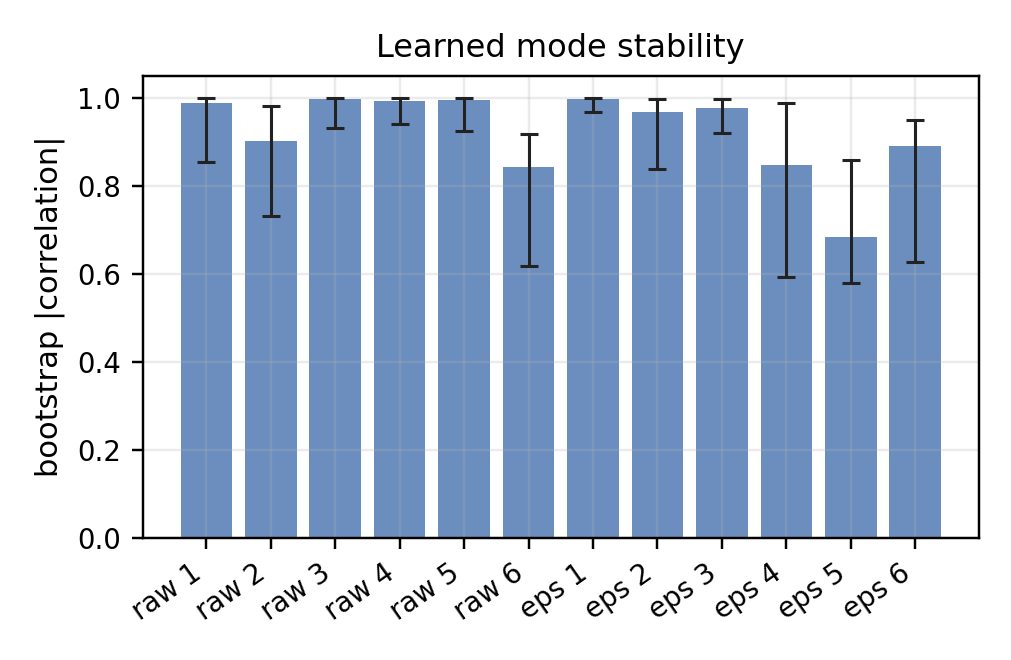
\includegraphics[width=\linewidth]{bootstrap_stability.png}
\caption{Bootstrap distribution of matched signed-mode correlations. The first
three modes are stable across galaxy resamples; the later modes have larger
sample sensitivity.}
\label{fig:bootstrap}
\end{figure}

The last check is whether the learned coordinates relate to diagnostics that
were not used in fitting. For
the signed residual-of-residual dictionary, coefficient 4 has correlation 0.413
with the binary central-overshoot flag and correlation $-0.592$ with the
continuous normalized inner-gap statistic. Coefficient 6 has the opposite
association with the overshoot flag (correlation $-0.371$). These associations
are not used in training; they indicate that the learned coordinates recover
part of the same structured failure mode found by direct NFW residual analysis.
Figure~\ref{fig:coefficients} visualizes this learned coefficient space.

\begin{figure}[t]
\centering
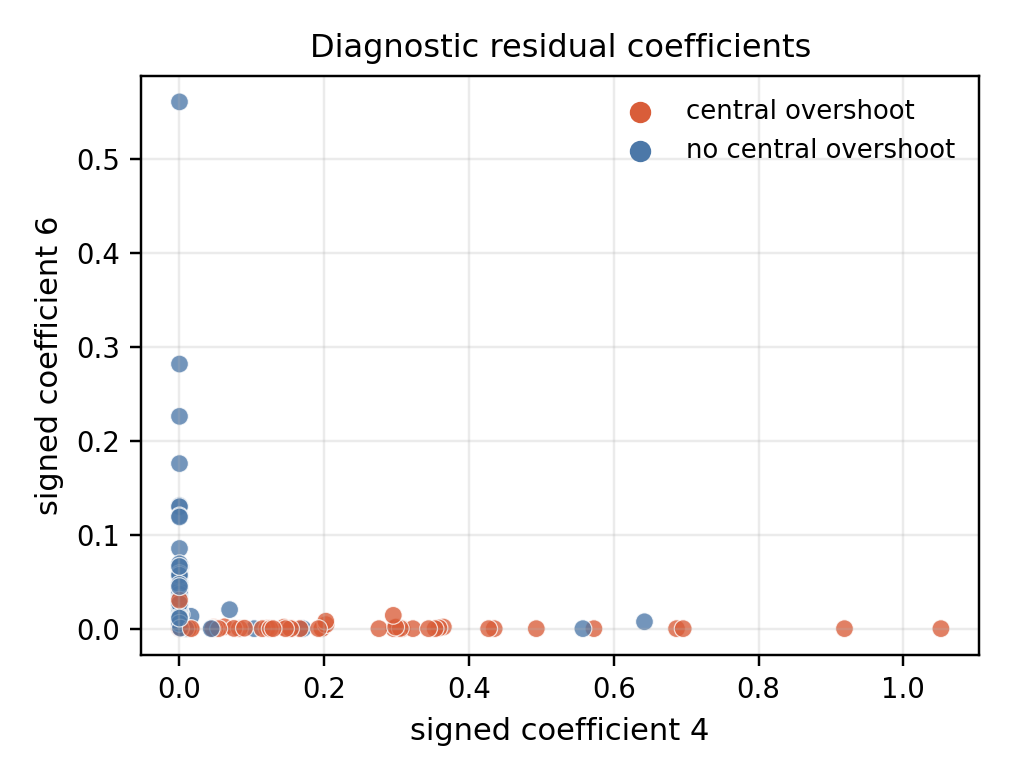
\includegraphics[width=\linewidth]{coefficient_space.png}
\caption{Signed residual-of-residual coefficient space. Points are galaxies;
learned coordinates recover population variation that aligns with independent
central-overshoot diagnostics even though those labels are withheld during
training.}
\label{fig:coefficients}
\end{figure}

\section{Discussion}

The contribution is statistical model criticism. It does not show that NFW is
wrong as a cosmological model, nor does it adjudicate between particle dark
matter and modified dynamics. The experiment uses fixed mass-to-light ratios,
simplified residual-space fits, no concentration prior, no baryonic feedback
model, and no marginalization over distance or inclination. A full halo
inference would require a richer likelihood and priors comparable to published
SPARC halo catalogs \citep{Li2020}.

The learning extension is therefore deliberately modest: learn the population
structure of the discrepancy, not the final source model. This keeps
the statistical task aligned with the inverse problem. If a mode is unstable,
it is probably a nuisance or a sample artifact. If a mode is stable, appears in
held-out radial entries, and correlates with independent residual diagnostics,
then it becomes a concrete target for physical modeling. A simulator,
field-equation surrogate, or baryonic-systematics model can be asked to
generate that mode rather than to explain every galaxy from scratch.

This framing also gives clear failure conditions. The result would be weak if
held-out reconstruction were close to the population mean, if bootstrap modes
could not be matched across resamples, or if learned coefficients were
orthogonal to all independent residual diagnostics. The present experiment
passes those checks for the leading signed modes but not uniformly for every
rank-six component. That is why the claim is deliberately about stable
population residual structure, not about a discovered six-component law of
galaxy dynamics.

The positive claim is that the residual left after fitting a physical baseline
has learnable population structure. This is useful for three reasons.
First, it provides a low-dimensional language for residual morphology, analogous
to dictionary learning in signal processing \citep{Olshausen1996,Aharon2006}.
Second, it separates baseline fit quality from repeated misspecification
patterns, in the spirit of posterior predictive checks and realized
discrepancies \citep{Gelman1996}. Third, it supplies a bridge to more ambitious
scientific machine-learning approaches: simulation-based inference could learn
which physical generators produce the observed residual modes
\citep{Cranmer2020}, while physics-informed models could add differentiable
field-equation constraints \citep{Raissi2019}.

The strongest near-term extension is held-out-galaxy validation. The present
held-out radial-point score tests whether profiles are compressible after some
entries are observed. A harder test is to predict the residual morphology of an
entire unseen galaxy from baryonic covariates, environment, or partial radial
coverage. Another necessary extension is uncertainty propagation over stellar
mass-to-light ratios, distances, inclinations, and NFW concentration priors.
If the stable signed modes persist under those perturbations, they become a
specific target for physical explanation.

\section{Conclusion}

Learning geometric residuals across SPARC galaxies turns a familiar
rotation-curve inverse problem into an interpretable statistical-learning
problem. A masked, smooth, nonnegative dictionary compresses both positive
observed acceleration residuals and signed NFW residual-of-residuals. The
signed dictionary is the central object: it learns coherent leftover fields
after a baseline NFW source has been fit to the outer galaxy. The first signed
modes are bootstrap-stable, and learned coefficients align with independent
central-overshoot diagnostics. The resulting stat.ML framing is simple: fit the
physical baseline, learn what remains, and use the learned residual geometry to
guide the next physical model.

\paragraph{Reproducibility.}
The experiment is implemented in
\texttt{experiments/sparc\_residual\_dictionary/}. It uses public SPARC
tables and the residual profiles generated by the companion SPARC
residual-of-residual pipeline, then writes all figures, CSV outputs, and the
Markdown experiment report used by this paper.

\small
\bibliography{sparc_residual_dictionary_learning}

\end{document}
